%http://texblog.org/2012/08/29/changing-the-font-size-in-latex/
\documentclass[12pt]{report}
\usepackage{amsfonts, amsmath, amsthm, amssymb}
\usepackage[urlcolor=blue,linkcolor=black,colorlinks=true]{hyperref}
\hypersetup{
  pdftitle = {A Novel Approach to Detecting Covert DNS Tunnels Using Throughput
Estimation},
  pdfkeywords = {},
  pdfauthor = {Michael Himbeault}
}
%\usepackage[headsep=1cm,headheight=50pt]{geometry}
\usepackage[dvips]{graphicx}
\usepackage{subfigure}
\usepackage{lscape}

% http://tex.stackexchange.com/questions/5091/what-to-do-to-switch-to-biblatex
% http://polyphys-s01.ethz.ch/images/bibstyles/
%\usepackage[natbib=true,style=numeric-verb,backend=bibtex]{biblatex}
%\addbibresource{../Reference/bibliography.bib} % Syntax for version >= 1.2
\bibliographystyle{amsplain}

\usepackage{setspace}
\doublespacing

\addtolength{\oddsidemargin}{-.5in}
\addtolength{\evensidemargin}{-.5in}
\addtolength{\textwidth}{1in}

\addtolength{\topmargin}{-.5in}
\addtolength{\textheight}{1in}

\newcommand{\hreff}[2]{\href{#1}{#2}\footnote{\url{#1}}}

\newtheorem{thm}{Theorem}[section]
\newtheorem{cor}[thm]{Corollary}
\newtheorem{lem}[thm]{Lemma}

\newtheorem*{hyp}{Hypothesis}

\theoremstyle{remark}
\newtheorem{remark}[thm]{Remark}

\theoremstyle{definition}
\newtheorem{definition}[thm]{Definition}

\theoremstyle{definition}
\newtheorem{example}{Example}[section]

\theoremstyle{definition}
\newtheorem{algorithm}{Algorithm}[section]

\begin{document}
\title{A Novel Approach to Detecting Covert DNS Tunnels Using Throughput
Estimation}
\author{Michael Himbeault}

\maketitle

% http://www.sce.carleton.ca/faculty/chinneck/thesis.html

% ==============================================================================
% The abstract should make sense to everyone.
% It should give them an idea of whether they possess the background necessary 
% to understand the paper, and if they do, what the paper will tell them.
% ==============================================================================
\abstract{In a world that runs on data, protection of that data and protection 
of the \emph{motion} of that data is of the utmost importance. Covert
communication channels attempt to circumvent established methods of control,
such
as firewalls and proxies, by utilizing non-standard means of getting messages
between two endpoints. DNS (Domain Name System), the system that  translates
text-based resource names into resource records, is a very common and effective
platform upon which covert channels can be built. This work proposes, and
demonstrates the effectiveness of, a novel technique that estimates data  
transmission throughput over DNS in order to identify the existence of a DNS
tunnel against the background noise of legitimate network traffic.
The proposed technique is robust in the face of the obfuscation techniques
that are able to hide tunnels from existing detection methods.}

\newpage
\tableofcontents
\listoftables
\listoffigures

\newpage

% ==============================================================================
% The introduction should make sense to people with the necessary background, and
% should be of moderate use to people without the necessary background. It should
% introduce the problem we are trying to solve, why it is worth solving, give a
% coarse picture of where our solution sits in the landscape of solutions, and 
% what the solution involves. It should briefly touch on the outcome of the 
% solution.
% ==============================================================================
\chapter{Introduction}

Control of the data that moves between hosts on a computer network is vitally
important in order to be able to enforce security policies and protect sensitive information. To this end systems
such as firewalls, proxies, and content filters are put into place in order to
monitor and control network traffic. Covert channels
are utilized to circumvent these control mechanisms for purposes that range from 
benign to malicious. This work focuses specifically on DNS tunnels, however
other types of covert channels do exist.

Detecting a DNS tunnel effectively on a busy network link becomes an exercise
in discrimination. Since there is such a wide variety of network traffic that
is generated on a busy link, there is generally no simple definition of
\emph{normal} for a particular class of traffic, including DNS. This tends to
either rule out, or decrease the viability of, algorithms that depend on
finding a definition of normal and alerting based on deviations from that norm.

A highly sensitive and specific detection of DNS tunnels on a busy network link
is an important problem in the arena of network security as it enables
administrators to block or otherwise control these potential sources of
compromise. A non-exhaustive, but informative, list of things that covert
channels (including DNS tunnels)
can be used for is:

\begin{itemize}
\item Data exfiltration
\item Communication through restrictive firewalls
\item Receiving commands or information from a remote source
\item Transport layer for complete VPN solutions
\end{itemize}

In enterprises that deal with sensitive information such as financial, health,
personal or intellectual property information it is of the utmost importance to
control the access to this information. Even if an enterprise does not have
information that needs protecting, DNS tunnels should still be blocked in order
to prevent malware from communicating. Because DNS tunnels can be used for
arbitrary communication, they can be used as command-and-control channels for
botnets or any other malicious system that relies on data transmission.
Preventing
botnets from operating is of the best interest for the Internet as a whole and
should be a concern of every user of the Internet.

Existing methods of detection rely on one of two methods, character frequency
analysis
and signatures, to detect the presence of a DNS tunnel. The signature-based
solutions attempt to identify portions of the tunnelling
application data (as opposed to the user data that is sent using the tunnelling
application) for which a signature can be built. These signature based
solutions are subject to many of the same problems that plague signature based
anti-virus solutions including their inability to detect zero-day situations.
 For example, if the application changes its communication
schemes, the signatures may no longer be valid and may no longer trigger when
they are intended and expected to. Additionally, signatures cannot be built for
applications
that are not available for study, or that aren't known of. For applications
that use a custom communication scheme that has not had a signature built
specifically for it, it is very likely that an existing signature will not be
relevant and will not detect it.

Because signature based schemes are not effective in detecting DNS tunnels in a
zero-day\footnote{\emph{Zero-day} refers to a situation where nothing is
known about the attack as it has never been seen or analyzed before.} situation,
another
method is required. Analysis based on character frequency is proposed
in\cite{Born2010.cfa} by Kenton Born with similar approaches proposed by several
other authors (see section \ref{litreview} for more details) which uses
character
frequency analysis under some assumed properties. More details are given in section
\ref{litreview}.

%that normal DNS traffic has a unique
%character frequency distribution that can be used as a discriminating
%fingerprint. Based on analysis of common domain names, he obtained a
%distribution that accurately describes normal DNS traffic while
%effectively detecting DNS tunnel traffic. Results obtained by Born indicate
%that DNS tunnels have an approximately uniform character frequency distribution
%whereas normal DNS queries do not.

A weakness of the approach proposed by Born is that it relies on the assumption
that DNS tunnel traffic \emph{necessarily} has a character frequency
distribution that is different from that of normal DNS queries. This assumption
is not necessarily true, and a proof-of-concept application
was developed that demonstrates this fact. The tool performs a
\emph{probabilistic encoding} that takes an arbitrary data source and encodes
it into a stream of characters that conforms to a given distribution. This tool
can be used to modify the output of any DNS tunnel application so that their
output conforms to the distribution that Born found for normal DNS traffic (or
any other distribution, for that matter). By
utilizing this transformation, Born's approach fails to detect the DNS traffic
as it becomes, from the viewpoint of his algorithm, indistinguishable from
normal DNS traffic. Details of this are given in section \ref{probencode}.

Due to the weaknesses listed above, it is clear that a new approach is
necessary that detects DNS tunnels in a zero-day situation and without the known 
weakness involving character frequency and probabilistic encoding. This work
proposes, and demonstrates the effectiveness of, a method of detecting DNS
tunnels that meets these requirements.

The proposed method operates under the assumption that DNS tunnels move more
data than a normal domain but don't necessarily do it by moving more bytes than
a benign domain. This distinction is important since, on a busy network, a large
content or service provider such as Google, Amazon, Facebook or Twitter may
comprise orders of magnitude more DNS traffic by byte count than a DNS tunnel.
By leveraging this fact, it is possible to detect
any use of DNS to transmit arbitrary data by measuring the amount of data that
is transmitted using a particular DNS domain or subdomain. The details of this
measurement methodology are contained in \ref{datameasurement} and requires
estimating the amount of unique data that is transmitted by analyzing the
queries themselves and not simply counting characters in the query string.

This proposed detection methodology is shown to detect DNS tunnels in as few as
ten packets and continues to be robust in highly hostile detection environments
such as those that contain a great deal of non-tunnel traffic as well as benign
uses of DNS for transmitting arbitrary data\footnote{Many security vendors
utilize the fact that DNS and UDP port 53 are so loosely controlled in order to
ensure that their deployed devices can communicate with the vendor intelligence
unimpeded.}. Detector performance on commodity hardware is shown to scale to
greater than two gigabits of UDP port 53 throughput per second, indicating that
this methodology does not sacrifice performance for detection accuracy and
remains practical for monitoring very large networks.

\newpage

% ==============================================================================
% The background section provides a reasonable breadth and depth of content for
% people to brush up enough to understand the literature review, problem at hand
% and solution. It should provide references for breadth and depth not covered
% in this section.
% ==============================================================================
\chapter{Background}

\section{Entropy}
Entropy is intuitively speaking, a measure of how random a particular collection
of items is. In the context of a random variable, entropy is a measure of the
uncertainty in the output of the random variable. A random variable that has a
distribution that outputs a particular symbol seventy five percent of the time
has considerably less uncertainty, and thus less entropy, than one that outputs
all symbols with equal frequency. In the context of a collection of symbols in a
stream, or data source, entropy can be though of as a measure of the information
content of that collection. If the collection comprises almost entirely a single
symbol, then that collection can be thought of as containing less information,
and thus having less entropy, than a collection where all symbols occur with
equal frequency.

Entropy can be calculated for a collection of symbols
$\mathcal{C}=\{c_1,\ldots,c_n\}$ with symbol $c_i$ appearing with proportion
$0\leq p_i\leq 1$ where $\sum_{i=1}^n{p_i}=1$ as

 \[H(\mathcal{C})=-\sum_{i=1}^n{p_i \log{p_i}}\]

The base of the logarithm determines the units of the resulting value. If a
logarithm in base 2 is used, then the entropy has the units of \emph{bits}, if
the logarithm with the natural base $e$ is used then the entropy has the units
of \emph{nats}, if the logarithm is in the common base 10, then the entropy has
the units of \emph{digits}.

\section{Domain Name System (DNS)}

DNS (Domain Name System) is the service through which names are mapped to
resources. Typically, this maps a name (such as \emph{www.google.ca}) to an IP
address. The value of this service is that names are considerably more
flexible, and considerably easier to remember, than the resource or record that
they point to. For example, \emph{google.com} is considerably
easier to remember than one of the IP addresses that it points to, such as
74.125.226.34. \emph{google.com} is also considerably more flexible, since it
points to not just one but several addresses, and successive responses
will receive different records in a round-robin, or random, fashion. This
rotation of responses allows for a crude form of load balancing and automatic
fail over, while retaining its ease of use.

The DNS protocol is assigned both UDP and TCP port 53 for
communication with most communication operating over UDP as opposed to TCP. The
use of TCP depends on the implementation of the resolver, however the
specification indicates the TCP should be used if the response data exceeds 512
bytes or during a zone transfer\cite{rfc1035}. DNSSEC (Domain Name System
Security Extensions), due to the fact that it requires a signature of
authenticity for all responses, will often cause the response to
require TCP\cite{rfc4034}. 
% http://www.iana.org/assignments/dns-sec-alg-numbers/dns-sec-alg-numbers.xml
Because there is no \emph{requirement} for when
TCP be used, some resolvers may be implemented to use TCP for all responses as
this does not violate the specifications for DNS.

The experiments related to this work do not consider the situation of DNS over
TCP since the analysis techniques are identical since the formats of the UDP
and TCP responses is identical once the TCP stream is reassembled. Modification
of the tools developed for this work would require the ability to perform TCP
stream reassembly in order to extract the responses from the TCP response.

Because DNS is such an integral component of Internet communication it is not
generally reasonable to simply block it while still expecting functional Internet
connectivity. A common approach is called DNS \emph{proxying} which
forces all DNS queries to be made to a DNS proxy server that is controlled by
the interested entity (ISP, company, etc...). This DNS proxy server is
responsible for handling all DNS queries for the internal network, and any DNS
queries that are destined for the Internet (as opposed to the proxy) are
typically dropped by the
firewall in this type of configuration. The DNS proxy server operates in
\emph{recursive mode}, which means that if a question is asked of it to which
it does not know the answer, the proxy server will then query for the answer (by 
issuing its own query to the global DNS system) and then respond to the initial
request using this response.

DNS is a heavily cached protocol due to how often data can be reused between
queries. Consider how often a desktop Internet user causes a request for
\emph{google.com}. If a request had to traverse the entire DNS system every
time, this would represent a very considerable amount of traffic being
generated. To avoid this, every DNS record has extra information about it that
includes, among other things, how long it can be cached for. Standard
caching lengths put it around one hour which means that a DNS server will only
recursively pass on a query for a record once an hour. This caching period is
not constant and can be set differently, depending on the information the
record contains. Some records require a considerably lower TTL (Time To Live),
as low as one minute, while for others a considerably longer (months) may be
appropriate.

This proxy architecture removes some naive operation modes for DNS tunnels
that will be discussed in in more detail in \ref{dnstunnels.types.raw}, but does 
not offer any protection against the more sophisticated forms of DNS tunnels.

\section{Covert Channels}

Covert channels are methods of communication that use non-standard means of
communication for the purpose of evading detection and/or blocking by the
existing security infrastructure. Covert channels may utilize
portions of an existing protocol or communication channel, or they may find
ways of transporting information utilizing a completely new medium. An example
of the latter is called a \emph{timing channel}, which can utilize the timing
between packets to convey information. A timing channel carefully controls the
timing between packets sent to a remote server to encode information, thereby
utilizing a method of communication that is not utilized by any
\emph{legitimate} protocol or communication method.

Covert channels come in may forms and not all types support the properties that
are normally associated with a communication channel. Because they are built on
unorthodox, or unreliable, transmission media and are subject to the effects of
intermediate routing and networking devices they cannot always offer all of the
same functionality as a legitimate channel.

Covert channels need not support bi-directionality due
to either the constraints of the underlying medium, or the effect of
intermediate devices. A covert channel that is only useful for reception is one
that utilizes a third-party image hosting service. It is possible to embed
arbitrary information into the header portion of an otherwise completely benign
JPEG image file which could then be posted to Facebook, Flickr, or any other
publicly accessible image hosting service. This image file can then be checked
by the remote
hosts to pull the information however, due to the nature of the image services,
the remote
hosts may have no
way of posting information back to the other endpoint, making the
communication channel unidirectional.

Real time data transfer refers to the ability
for a communication channel to send data immediately. UDP, by its very nature,
supports this and TCP supports this via the PUSH flag which indicates that data
is being sent before a full window has been accumulated. The TCP PUSH flag
is used, for example, during an SSH connection in order to provide
interactivity. Timing channels, or any channel that relies on modifying normal
system traffic instead of generating their own traffic, by their nature, are
unable to support real time data transfer. This is because they need to wait for 
a system packet in order to send their data, and if the system goes for a period 
of time without sending data then the covert channel must wait as well.

\section{DNS Tunnels}
\label{dnstunnels.types}

DNS tunnelling is the method by which arbitrary data is made to be transferred
over the same channels as DNS. DNS tunnels come in one of two types: raw, or
conforming.

\subsubsection{Raw DNS Tunnels}
\label{dnstunnels.types.raw}
Raw DNS tunnels do not attempt to mimic or conform to the DNS
specifications, and simply attempt to utilize the fact that UDP port 53 is
often left open in firewalls. Raw tunnels attempt to exploit this by
transmitting arbitrary traffic using UDP port 53 packets with arbitrary payload. 
This is the most efficient exploitation of the ubiquity of DNS as it incurs the
lowest amount of overhead, both computationally and in terms of network
throughput. The trade off for this efficiency is that it is the least
conforming and the most likely to get stopped by either a firewall or a proxy.
In the situation where all DNS queries are forced to be proxied through a
dedicated DNS server, raw DNS tunnels will fail to operate as expected. This is
because when the UDP port 53 traffic is redirected to the proxy, the DNS server
will attempt to interpret the arbitrary payload as a DNS packet and will likely
fail. When it fails, it will drop the packet thereby preventing all raw UDP
port 53 communication. Because these types of tunnels are effectively blocked by 
standard firewall and proxy practises, detection of these tunnels is not
considered in this work.

\subsubsection{Conforming DNS Tunnels}
\label{dnstunnels.types.conforming}
Conforming DNS tunnels produce DNS packets that conform to all appropriate
specification and RFC documents and, as far as any DNS server, is concerned the
traffic generated is valid DNS traffic. These tunnels incur the highest
computational and throughput overhead, but have the advantage that detecting
and blocking them is a very difficult process. The detection of this type of
DNS tunnels is the topic of this work. This type of tunnel is capable of
operating, even in an environment with very strict firewall and proxy policies.
Because this type of tunnel operates in very hostile (to the operation of the
tunnel) environment, detection of this type of DNS tunnel is of interest to all
levels of government and industry.

Conforming DNS tunnels operate by embedding the data for transmission into the
query string and the response and require a modified, non-conforming, DNS
server on one end of the connection and a piece of software on the client end.
Typically these types of DNS tunnels have one endpoint that is controlled by the 
tunnel user, with that controlled endpoint running dedicated server software
that. The client and server software is responsible for transforming arbitrary
information into DNS queries, and for translating DNS responses back into the
arbitrary data that it represents. The precise details of how the translation
is done between DNS and the raw data depends on the implementation.

\subsubsection{DNS Tunnel Software}

Some DNS tunneling software is OzymanDNS\cite{ozymandnssrc},
Iodine\cite{iodinesrc},
Dns2tcp\cite{dns2tcpsrc},
DNScat\cite{dnscatsrc} and
DeNiSe\cite{denisesrc}, and
PSUDP\cite{psudpsrc}. Each of these have
slightly different operational characteristics, but they all aim to do the same
thing, which is transmission of arbitrary data over DNS.

Iodine supports raw tunnels, as well as moving information back from the server
in A (IPv4 addresses), MX (mail server), TXT (arbitrary text) and may other
supported DNS record types.TXT records are rarely used by
consumers or end-user applications, and so a blanket block policy of TXT
records for end-user devices would have very little impact on end-user
applications. TXT records are as close to a raw tunnel that a conforming
tunnel can get to in terms of throughput.

DNScat utilizes CNAME (alias to
another record) records and a supplementary A record, when appropriate, however
the A record is not actually used for throughput. OzymanDNS and DeNiSe utilize
solely the
TXT record, which is as close to the raw tunnel as possible, however can be
easily neutered by simply blocking TXT records. Because these tools only uses
TXT records it is possible that it is the least flexible and deployable out of
those listed above given a hostile environment. Dns2tcp utilizes either TXT or
KEY records, which makes it as flexible as OzymanDNS and DeNiSe. The KEY DNS
record was designated for specific uses\cite{rfc2931}, but has been
deprecated now\cite{rfc3445} in favour of the DNSKEY record for use with
DNSSEC\cite{rfc3755} and the IPSECKEY for use with
IPSEC\cite{rfc4025}. Because of this deprecation, use of the KEY record is
subject to strict filtering which greatly reduces the effectiveness of this
solution.

All of the above tools utilize encoding and decoding mechanisms that would
successfully propagate through a proxy server, at the cost of the fact
that the tunnel applications have to generate their own traffic. PSUDP, 
proposed by Kenton Born, aims to remove the latter requirement by creating slack space
within an existing DNS packets at the UDP transport layer. He proposes two ways
of creating this slack space: naively placing it at the end of the packet, and
rearranging the DNS query string to utilize pointers to create this
slack space in the middle of the packet. Pointers allow
for the re-use of DNS query strings within a packet to save on space. They are
an optional component of the specification, but allow for considerable space
savings. A pointer in a DNS packet is a special sequence of bytes that
indicates where in the packet the processing of the query string should jump
to. When processing a query string, only a single pointer can be followed,
according to spec, which prevents multiple redirection and infinite loops
(where a pointer points to itself). By having a pointer point forward in the
packet, it is possible to cause the parsing of a query string to skip a number
of bytes, creating slack space.

This method relies on this slack space, which is not parsed by normal servers
or clients, but can be contain arbitrary data that is extracted by special
clients. However, because this slack space is not processed by DNS servers, in
an environment where all DNS queries must go through a proxy, this method is
incapable of producing a covert channel that is able to penetrate a strictly
proxied DNS environment.

\newpage
\chapter{Review of the State of the Art}
\label{litreview}

The solutions that exist to date generally make very little use of complex,
static, signatures but rather attempt to exploit a characteristic trait or
property that the DNS tunnel will exhibit. If a tunnel can be crafted to not
exhibit that feature, then those detection strategies will normally fail in
their detection. This section summarizes the known detection methods, their
commonalities, advantages, and disadvantages. It will then take the body of
detection methods as a whole and establish the existence of any gaps, or
weaknesses, that could be exploited by an application to circumvent an IDS that
made use of \emph{every one of the mentioned detection methods}. This
essentially identifies gaps in the current state of the art that could be filled
by a new technique, or an adaptation of an existing technique.

\section{General Covert Channel or Anomaly Detection Research}
(Browne, 1994)\cite{Browne1994} establishes an entropy conservation based
approach for testing the completeness of general (that is, not specific to DNS)
covert channel analysis and detection methodologies. (Shaffer,
2008)\cite{Shaffer2008} Proposes a Security Domain model for assessing the
surface of a piece of software for exploitable covert channels.

(Ray, 2008)\cite{Ray2008} proposes a protocol for use in a covert channel that
incorporates stealth, low overhead, data integrity, data confidentiality, and
data reliability. The protocol can be used on top of any other covert channel
transport method (ICMP, IP, HTTP, DNS, etc\ldots)

(Horenbeeck, 2006)\cite{Horenbeeck2006} discusses, briefly, DNS tunnels and
their implications. A short mention of proxying DNS requests is given as a
potential solution but without examining the multitude of ways that a DNS tunnel
could still operate in such an environment. The rest of the paper discusses the
risk management and policy based mitigations that can be applied to covert
channels in general.

(Moskowitz, 2003)\cite{Moskowitz2003} investigates the link between anonymity
and covert channels. It identifies several linking factors such as covert
channel capacity and the properties of anonymizing networks, and investigates
how these affect anonymity of participants in a communication.

(Newman, 2007)\cite{Newman2007} discusses covert channels in a broad sense,
examining the various types of covert channels along with the relationship
between covert communication, cryptography, steganography and secrets.

(Okamura, 2010)\cite{Okamura2010} discusses a fascinating type of covert channel
for communication between virtual machines that share a physical host. The paper
proposes that virtual machines can manipulate their CPU core load, which is
peripherally visible to other virtual machines on the host, in order to send and
receive information.

\section{Non-DNS Related Research}
Tunnel Hunter\cite{Dusi2009} is an application that aims for general covert
channel detection over a variety of tunnelling communication channels.

(Bauer, 2003)\cite{Bauer2003} discusses a new type of HTTP-based covert channel
that adds the unwitting web browser application to the anonymity set.

(Borders, 2004)\cite{Borders2004} discusses a method of detecting data egress
using HTTP-based covert channels.

(Cabuk, 2004)\cite{Cabuk2004} and (Cabuk, 2009)\cite{Cabuk2009} discuss the
design and detection of IP (Internet Protocol) based covert timing channels.
(Gianvecchio, 2007)\cite{Gianvecchio2007} discusses an entropy-based approach to
detecting covert timing channels on the Internet based on their effect on the
original process' entropy properties.

\section{DNS Covert Channel Research}
The SANS Institutes's InfoSec Reading Room published a report on the design and
detection of DNS tunnels\cite{SANS2013}. The report covers a very wide variety
of topics including background information, tunnel-specific information,
technical information, existing applications, detection techniques, detection
implementations, and a sample detection scenario. This report is exceptionally
good reading as a primer on the topic. The sample detection scenario employs an
analysis technique very similar to the technique that will be outlined in
section \ref{datameasurement}.

(Karasaridis, 2006)\cite{Karasaridis2006} proposes and evaluates mechanisms that
use network flow data\footnote{Flow data is a way of digesting network packet
data into information per communication, stream, or (in the case of UDP since
there is no inherent concept of a stream of interrelation of packets) temporally
contiguous collection of packets.} to detect DNS anomalies including cache
poisoning and tunnels. Their detection of DNS tunnels involves estimating
average packet size distributions over a given time interval (in the paper
hourly distributions were produced), and then comparing the actual distributions
with a baseline distribution using cross-distribution entropy computation. The
authors are able to observe considerable changes in their cross-distribution
entropy measurement during the onset of the Sinit virus in their real-world
data. This approach is discussed in additional detail in (Roolvink,
2008)\cite{Roolvink2008}.

(Born, 2010)\cite{Born2010.exfil} discusses a way of using javascript in a web
browser to exfiltrate data from a network, while \cite{Born2010.psudp} discusses
a novel way of crafting a DNS tunnel that exploits the nature of a DNS packet
and the ability to create unused space in the packet in which arbitrary data can
be stored. \cite{Born2010.cfa} discusses a method of detecting DNS tunnels by
examining character and $n$-gram frequencies in the names that are being queried
for. \cite{Born2010.ngviz} demonstrates the effectives of data visualization
when attempting to detect a DNS tunnel using a custom visualization engine using
the character frequency analysis proposed in one of the Born's previous
publications. If a DNS tunnel can be crafted such that its character frequencies
are distributed sufficiently close to those of legitimate DNS names, then it is
possible to hide a DNS tunnel from this type of analysis.

(Butler, 2011)\cite{Butler2011} demonstrates a way of quantitatively analyzing
covert communication channels with particular focus on DNS covert channels. It
proposes a \emph{codeword mode} of communication over DNS where a specific
lexicon is chosen that allows the two endpoints to communicate with. Each word
in the dictionary has a particular meaning\footnote{The words can represent
binary information, or can represent higher level constructs such as commands in
the context of a botnet or piece of malware.} that is understood by both
endpoints. This lexicon must be chosen \emph{a priori} and must be common to all
endpoints wishing to communicate using this method. Butler also discusses the
concept of perfect stealth of a covert channel based on DNS, and proposes a deep
packet inspection based countermeasure that utilizes the \emph{Jensen-Shannon
divergence} measure. The method relies on an assumption very similar to that in
Born's character frequency analysis where the tunnelled traffic uses DNS names
with a measurably different character distribution than that of legitimate DNS
traffic. Because of this similarity of assumption this approach suffers from the
same vulnerability as Born's.

(Romana, 2007)\cite{Romana2007} discusses their analysis of DNS data on a large
campus network. They use the output of a DNS resolver's query logging as their
input, but the process works just as well on other inputs even though they
aren't discussed. Digestion of the large query log file is done with standard
Unix utilities and logic available on almost all Unix-based systems. The authors
estimate the entropy of the source IP address (of the DNS query) and teh queries
themselves, and perform analysis based on that output. The scalability of this
approach is not discussed in detail, nor is an adaptation of it to consider more
refined sets of queries since this approach only takes all parts of all queries
together for analysis. Adaptation of this approach for real-time analysis is not
discussed either. Because this approach is does not discriminate with respect to
finely grained slices of time, nor to domain or subdomain information, it
necessitates that all of the query data be kept around for postmortem analysis.
The approach is able to alert to the fact that something was detected, but it
cannot indicate precisely when, indicate in a timely fashion, nor can it give
any indication as to what caused the alert. These details must be ascertained
from the raw query data after the proposed approach throws an alert which
increases response time and the manpower required to investigate an alert.

(Thomas, 2011)\cite{Thomas2011} proposes and evaluates the efficacy of an FPGA
(Field Programmable Gate Array) based solution for detecting malicious DNS
packets on a high throughput network link. The work extends prior work to
including more flexible detection and to support more current-generation network
infrastructure (the previous work was limited to 100Mbit network connections,
with the new work operating on 1000Mbit network connections). The fact that this
approach makes use of specialized hardware makes it prohibitively complex for
smaller companies to implement and use. The analysis performed on the DNS
packets in order to determine their validity is done via a signature-based system
where the DNS query is hashed, and the hash is compared to a blacklist of
domains that are disallowed due based on the network policies. Because this is
signature and blacklist based, this approach suffers from the standard problems
such as weakness against zero-day situations and the inability to be agile in
the face of an adaptive attacker\footnote{In this case, if the attacker chooses
to use a new domain, the tunnel will succeed since the system does not have the
new domain on its blacklist yet. Similarly, if an attacker is using a publicly
available domain for their tunnel, the blacklist can affect other legitimate
traffic on that domain.}. The tests of this system use highly synthetic testing
methods that do not involve real-world data or synthetic data that attempts to
resemble real-world data.

(Dietrich, 2011)\cite{Dietrich2011} examines the use of DNS for command and
control of botnets based on the reverse engineering of the \emph{Feederbot}
botnet application. Based on the lessons learnt from Feederbot, the authors
applied their methods to other real-world traffic and detected other botnets
that also use DNS as their command and control medium. The authors make use of
two different approaches for classifying malicious DNS traffic from benign and
legitimate traffic. The first approach makes use of entropy calculated over the
responses DNS queries, very similar in theory to the character frequency
analysis proposed by Born\cite{Born2010.cfa} and is vulnerable to the same
methods of circumvention\footnote{That is, if the botnet architected the data in
the examined fields to conform to the author's model of benign traffic, then the
botnet could effectively masquerade as benign traffic and become invisible to
this method of detection.}. This portion of their approach operates a single
packet at a time, and does not consider aggregate information. The authors also
propose the use of behavioural analysis on data and statistics gathered from the
aggregate of several packets to estimate the persistence of DNS queries as well
as the amount of data moved over DNS by each host on the network. The
persistence of the connection is estimated by considering the maximum time
between DNS packets whereas the throughput over DNS is measured by counting the
bytes in all of the data segments of response packets and summing over time. The
persistence analysis can countered by a botnet that models its communication
with the command-and-control server based on a Poisson distribution with
inter-packet times imitating that of legitimate traffic. Similarly, the
throughput analysis can be countered by employing codewords and rate limiting to
utilize a high-level protocol compression to reduce the amount of data that
needs to be sent, and to reduce the amount of data actually transmitted in a
given time period to reduce the footprint of the bot on the network.

(Paxson, 2011)\cite{Paxson2011} is a slide deck that discusses the author's
searches through large campus networks for DNS tunnels in the wild. The author
proposes an approach for detecting DNS tunnels that is very similar to the
method proposed in this work in that it examines the approximate amount of data
transferred per domain and/or subdomain. The author, instead of utilizing
entropy measures, makes use of the utility \emph{gzip}\footnote{gzip is a
compression library that is used to compress input streams such as archives or
other files.} to estimate the amount of data moved under a domain in a given
collection of queries. The author's assumption is that gzip already is optimized
for compressing data, which can be thought of as measuring the amount of unique
data that is contained in the uncompressed stream. The author also mentions the
codebook/codeword method of embedding information into DNS queries, similarly as
to what was discussed in \cite{Butler2011}. The author successfully applies this
approach to real-world data and identifies DNS tunnels that were previously
unknown. The author, however, defines absolute thresholds for use in detecting
which domains classify as being a tunnel as opposed to comparing the data moved
from each domain to its peers and performing a more relative and context-aware
analysis. The utilization of the gzip algorithm reduces the scalability of the
approach due to the computational overhead incurred, limiting the applicability
to smaller networks or postmortem (as opposed to real-time) analysis.

jhind\cite{jhind2009} gave a presentation at DefCon 17 that discusses the use of
artificial neural networks to identify DNS tunnel traffic. The author proposed
that the neural network operate on the euclidean distance between the various
queries to a particular subdomain, treating the queries as vectors in higher
dimensional Euclidean space. The author successfully detected DNS tunnels as
produced by several software packages (Iodine, Ozymandns and Dns2tcp) using the
described approach. The approach outlined by the author suffers from the normal
training problems associated with neural networks, such as over or under fitting
to the training data, which may or may not prove to be problematic in the real
world. The author does not go into detail about the accuracy and precision of
the neural network which is very important for real-world applications where
false alarms and false negatives are costly errors. Additionally, it is
theoretically possible for a DNS tunnel to encode its outputs using a codebook
where every word has a distance from every other code word that is within a
desired range. Such a codebook could constructed by including all words that,
when treated as vectors in $n$ dimensional Euclidean space, lie within a ball of
radius $r$ where $r$ is the maximum desired distance. By doing this, it is
possible for a tunnel to fit within the neural network's definition of normal
and to pass by undetected.

Jeffrey Guy blogged in 2009 about visualization as an aid for detecting DNS
tunnels by looking at frequency and request/DNS name length plotted together. In
the concluding portions of the article the author mentions briefly, and in
passing, that the count of the number of different host names per domain could
be of value. The provides no further discussion of this topic, however, and
leaves it as an anecdote to the article.

Static signatures exist for at least three common network anomaly detection
engines (Snort\cite{Chamberland2009.snort_iodine},
Proventia\cite{Proventia2013.ips_tunnel}, and TippingPoint\footnote{TippingPoint
does not make information about its filters available as public information,
however correspondence with a TippingPoint user revealed that filters 9932 and
9938 trigger on the application data contained in DNS packets generated by
Ozymandns.}) engines, with others likely offering similar functionality. It is
important to note that these filters and rules do not trigger on all DNS
tunnelling applications and may not be robust in the face of a zero-day
situation.

\section{DNS Tunnel Detection Landscape}
\label{litsummary}
Taken together as a collective body of work, the detection approaches for DNS
tunnels can be summarized as follows, with the weaknesses and strengths of each general approach outlined.

\begin{itemize}
\item Signature based approaches exist for several popular detection platforms.

\textbf{Strength:} The fact that the platforms are common and already deployed
makes it very easy to deploy these signatures to a large number of existing
networks.

\textbf{Weakness:} The static nature of the signatures means that they are not
flexible enough to effectively identify more than a small portion of the
available tunnelling tools.

\item A detection method based on flow data, which offers a more scalable
approach due to the reduced amount of information that needs to be processed, is
proposed which examines average packet length and statistical deviations thereof
compared to a normal baseline.

\textbf{Strength:} This approach is flexible in that it is not limited to
looking at characteristics of particular applications, but rather at patterns of
behaviour that may be exhibited by any DNS tunnel.

\textbf{Weakness:} This approach assumes that DNS tunnel software will exhibit
longer packet and query lengths than normal traffic which is not necessarily
true. DNS tunnels can use carefully constructed encodings to ensure that their
queries stay small enough so as not to stand out against benign and legitimate
traffic. Simply limiting the size of their queries will not suffice, since the
proposed detection algorithm relies on comparing the distribution to a known
normal distribution, however carefully choosing the length of the queries such
that they satisfy the normal distribution will allow the tunnel to remain
undetected. Further, since this approach relies on identifying a baseline, it is
not necessarily suitable for links with a high variability of traffic patterns
(perhaps due to time-of-day variability, or where it is not feasible to
determine if the chosen normal baseline contains malicious traffic or not) where
false alarms and false negatives may become common.

\item The use of artificially created slack space in a packet is a novel
approach with a great deal of flexibility for creating a DNS tunnel.

\textbf{Strength:} The slack space requires application aware inspection that
performs deep packet inspection to determine the existence of, and then the
contents of, the slack space.

\textbf{Weakness:} This type of DNS tunnel has a crucial weakness in that this
slack space is not processed by recursive resolving DNS servers, and such will
not persist past the first resolver in a chain in such an environment. If these
packets are not sent directly to the DNS tunnel server endpoint, the payload
will not survive and the tunnel will not operate. Because of this, no special
detection or analysis mechanisms are required, and a simple DNS proxy will
suffice in preventing these types of tunnels.

\item A form of character frequency analysis is used in several approaches to
detect the existence of DNS tunnels.

\textbf{Strength:} This approach makes use of the assumption that DNS tunnels
produce queries and/or responses with a measurably different character
distribution than that of benign traffic. Since this assumption is quite
general, it applies to any DNS tunnelling application.

\textbf{Weakness:} Because this approach relies on the assumption that the
distributions are measurably different, if a DNS tunnel were able to construct
its queries such that its character distribution matched the expected
distribution, then it would be able to evade this type of detection. A
proof-of-concept approach and software application are presented in section
\ref{probencode} that is able to perform a loss-less two-way coding from a high
entropy source (such as compressed or encrypted data) to a stream whose
character frequency matches any\footnote{There are some small caveats that are
explained in detail along with the rest of the algorithm.} given distribution.

\item Hashes and blacklists are used along with an FPGA based implementation of
the algorithm for analyzing DNS traffic and blocking packets deemed to be
malicious.

\textbf{Strength:} This approach, due to its fast hashing algorithm and FPGA
based implementation, scales to very high throughput.

\textbf{Weakness:} Due to the blacklist nature of this approach, it suffers from
the same vulnerabilities as other signature based methods; inability to react
intelligently to a zero-day situation or clever adversary. Further, since it is
built on highly custom hardware requirements, it is not always practical for
smaller network operators to deploy.

\item A few approaches examine the behaviour of DNS tunnels and their effects on
the statistical properties of the queries themselves over time. These approaches
consider very similar approaches to the one given in this paper, explained in
detail in section \ref{datameasurement}.

\textbf{Strength:} These approaches are considering the most fundamental source
of information for a DNS tunnel; the queries themselves. Because DNS tunnels use
the queries as their communication, it makes the most sense to attempt to
examine these queries for the keys to detecting the tunnels.

\textbf{Weakness:} The weaknesses of the techniques proposed in the existing
literature include cleverly constructed queries (such that they sit within a
ball of a desired radius in $n$ dimensional Euclidean space), they are not
suitable for real-time analysis (such as the use of higher overhead measuring
mechanisms like gzip) or they do not discriminate between different domains
or subdomains.
\end{itemize}

\newpage
% ==============================================================================
% The problem statement should state the problem, and give context as to its 
% importance. It should explain the problem in terms of the information covered
% in the background. It should set the benchmarks for determining success or 
% failure of the new method, ideally in terms of a comparison to an existing 
% method, or the ability to pass a certain statistical test (desired traffic 
% should be picked out compared to real-world traffic with some reliability 
% measure).
% ==============================================================================
\chapter{Problem Statement}

\section{Brief Statement}
\label{briefproblem}
The purpose of this work is to investigate the feasibility of real-time DNS tunnel detection that does not suffer the common weaknesses of existing techniques.

\section{Detailed Problem Description}
DNS tunnel detection is a complicated task made worse by the fact that DNS
tunnel traffic can appear to be completely legitimate network traffic that
conforms to all standards and restrictions. It
need not violate any established standards or conventions, which makes it
difficult to detect against the background of normal DNS traffic based on
testing for violations.

This property of DNS tunnels makes them a particularly effective transport
mechanism
when data exfiltration or network control circumvention is the end goal. For
this reason an efficient method of detecting DNS tunnels is required that can
effectively detect a DNS tunnel against normal DNS traffic with a low
false-positive rate and that must not be susceptible to existing methods of
circumvention.

From section \ref{litreview} it is evident that there are currently several
approaches to detecting DNS tunnels that are not signature based as well as
signature based approaches of varying flexibility. There is only one mention of
performing real-time analysis at the domain/subdomin level, and it is anecdotal in nature
with no clear analysis of its merits or validity. The only other similar
approach involves aggregating all domains together and taking their queries
together for analysis which obliterates any per-domain statistics that could have been gathered.

Looking at this landscape, it becomes evident that there is a highly advanced theoretical
DNS tunnel that could evade all of the proposed real-time detection techniques.
Any detection that may occur postmortem would not be
able to alert to the threat in an adequate time frame to stop the attack in
progress. This tunnel would have the following traits:

\begin{enumerate}
\item All of its DNS packets would conform to all appropriate DNS RFCs.
\item Its queries would be chosen such that the character frequency distribution
matches benign DNS queries (to evade \cite{Born2010.cfa} and similar approaches).
\item Its queries would be chosen such that they have a distribution of lengths that
matches benign DNS queries (to evade \cite{Karasaridis2006} and \cite{SANS2013}).
\item Its queries are chosen such that they do not span too great a space when taken as vectors in higher dimensional Euclidean space (to evade \cite{jhind2009}).
\end{enumerate}

Item one is already demonstrated in practise by most of the tunnelling
applications available, and item two is shown to be possible in section
\ref{probencode}. Item three is easily accomplished by simply splitting queries based on a statistical model of the desired lengths, and item four will be shown in section \ref{querydistance} to approximately follow from item two based on empirical measurements.

\section{Solution Evaluation Criteria}
The objectives that must be met for an approach to have successfully solved the problem posed in section \ref{briefproblem} are as follows:

\begin{itemize}
\item Successfully discern both synthetically generated tunnels and known tunnels
in real-world data from normal, benign, DNS traffic.
\item Be resistant to known obfuscation methods compared to existing detection
methods.
\item Be able to operate at high speed on general purpose, easily obtainable
hardware.
\end{itemize}

The proposed approach will be evaluated against these criteria to determine
whether or not it can be considered an improvement on the state of the art for
this type of detection.

\chapter{Proposed Detection Method}
\label{datameasurement}

The method proposed in this work examines the information theoretical properties of the
DNS queries to each subdomain, thus retaining the flexibility to filter and
alert per domain as opposed to more generally on the set of all DNS queries. The tools developed to test this approach utilize full packet data for its analysis, but can be modified to use name server query logs (as were used in \cite{Romana2007}) or other sources of query information. The prototype software is easily capable of running at greater than gigabit speed on inexpensive, off the shelf, hardware making this approach inexpensive to deploy on smaller networks or in resource constrained situations.

\chapter{Demonstration of Existing Weaknesses}
This section will demonstrate that the weaknesses listed in section \ref{litsummary} are in fact exploitable by software and are not simply theoretical in nature.

\section{Probabilistic Encoding}
\label{probencode}
Several detection methods in the literature involve examining the character distribution in the queries, or responses, of DNS packets. These approaches compare the distributions obtained from the traffic being analyzed, and compare them to a known distribution that can be considered normal. If there is a sufficiently significant measurable difference, then the packet is flagged as anomalous.

If it were possible for a DNS tunnel to encode its output in order to match the distribution that these detection methods consider normal, then it would be possible for it to evade detection by masquerading as benign DNS traffic. These detection methods assume that the output of a DNS tunnel will have high entropy (due to compression and/or encryption) and/or span a wide range of character values, whereas normal traffic does not have these features. The solution to this problem becomes one of encoding a high entropy source into a lower entropy encoding in a way that the high entropy stream can be recovered from the low entropy encoding, where the low entropy encoding has a specific distribution of characters.

A proof-of-concept tool was written in C that performs precisely this task. The tool takes, as input, what it assumes to be a high entropy source\footnote{Since any source can be used to produce a high entropy source through encryption or compression, this is considered a safe assumption and limitation.} and a configuration file that describes the desired output distribution.

\subsubsection{Sample Encoding}
A sample encoding is given using the english character frequency distribution with the character distribution table used given in Table \ref{TABLE_unigrams}. In order to ensure that interested parties can verify this output, the source high-entropy data is contained in Table \ref{TABLE_encodingsource}. A data matrix image of the same base64 encoding is also given in Figure \ref{FIGURE_encodingsource}. This can be converted back to the original source via the standard Unix command line tool \emph{base64}. The output of the encoder using english character frequencies and the given input data is shown in Table \ref{TABLE_encodingoutput-unigram} which is clearly not english to any human observer or any analysis tool with knowledge of English di- and tri- gram frequency information.

\begin{table}
\centering
\begin{tabular}{ | c | c || c | c | }
Character&Count&Character&Count\\
\hline
$<$\emph{space}$>$&0.11965  &  u&0.0242803\\
e&0.111823 &  m&0.0211814\\
t&0.0797253&  w&0.0207765\\
a&0.0718989&  f&0.0196144\\
o&0.0660886&  g&0.0177392\\
i&0.0613258&  y&0.0173783\\
n&0.0594154&  p&0.0169821\\
s&0.0557003&  b&0.013135\\
h&0.0536491&  v&0.00860991\\
r&0.0527071&  k&0.00679637\\
d&0.0374417&  j&0.00134695\\
l&0.0354345&  x&0.00132054\\
c&0.0244916&  q&0.000836341\\
       &    &  z&0.000651466\\
\end{tabular}
\caption[English character frequency]{Probability distribution used for english character frequency in the sample encoding and decoding.}
\label{TABLE_unigrams}
\end{table}

\begin{table}
\begin{verbatim}
HEzQcP9uxPOzeOB1SfRP+DQ7x3X5dTA1WF3vpcnO5kgLQQEP7xnUrnUy7U8ISNdbNQd+8da64+Ci
nNBRvu3TRlG0KJvLzb6QDBWqxVfa4VeAU+cSvj+uzoajp2F0jd5/csHxJQlguoeqT76pq8oStoLG
3k48PZWuebgweZx5KdxAgUfN7/kvzwBzG7O+9B7J/O8y6BfGz6In0H+LuDCOsFqMljljX3SkgJq/
yPka52SDxa3D4GXecj9d
\end{verbatim}
\caption[Encoding sample - source]{The base64 encoding of the binary data used for the sample encoding.}
\label{TABLE_encodingsource}
\end{table}

\begin{figure}
\centering
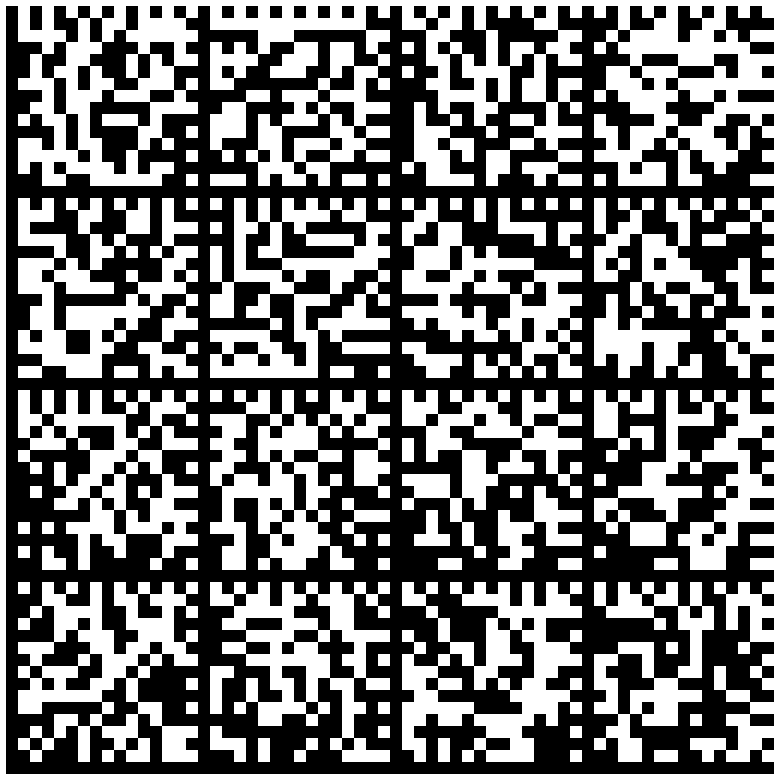
\includegraphics[width=4in]{figures/encoding_source.png}
\caption[Encoding sample - source (data matrix)]{The base64 encoding of the binary data used in the sample encoding, represented in a data matrix image.}
\label{FIGURE_encodingsource}
\end{figure}

\begin{table}
\begin{verbatim}
" mfeo  hnhaeeeewsao os eewk es fsemroh eeeewthesdre s sol sreese ea hrzltse
wesrnyemnpaoonef  ht   hsheawnfdemue stntleewth    home esaiu s feesgealne seaoa
hlhyp hmb ewaaeesdubotongtnploaanewefochd htugeside s oeesi   fptsmr
hweeeesoltsnahao esde hgmuo weeeeewyl  haoesroo     frmeshtieest ewad svikefui
hnceslphstestidau eeahl hrosoan wrthaa ft  heabpeeses eeeeewrsn    hrlucne ewr
esesooc eeeeeewsqe eewefgeesng est f eeeeewlhhae hgao hiuggnrrancewgmob
hdreeesgopesuoamyufiolisx esrrsloaeewtse"
\end{verbatim}
\caption[Encoding sample - output]{The encoded form of the binary data according to English character frequencies.}
\label{TABLE_encodingoutput-unigram}
\end{table}

% Efficiency numbers
% ==================
% Unigram
%   Efficient 0.417057 v 256946 0.06682579831758034750036661712845
%   Accurate 0.300548 v 332774 0.00014558032328364780948779390679
% Digram
%   Efficient 0.410661 v 270396 0.90056751440933662212073829206813
%   Accurate 0.280415 v 355834 0.0021880889

Analyzing the frequencies of the output shows that it closely approximates english character frequencies. A larger sample of random data (one hundred thousand bytes) was also encoded, and its output analyzed as well. The small sample, the large sample, and actual english character frequencies are displayed together in figures \ref{FIGURE_frequencies-bytop} and \ref{FIGURE_frequencies-bychar}. As is evident from the combined plots of the various distributions, there does not exist a clear distinction between them and thus it becomes very difficult to perform automated classification when information is encoded using this tool.

\begin{figure}
\centering
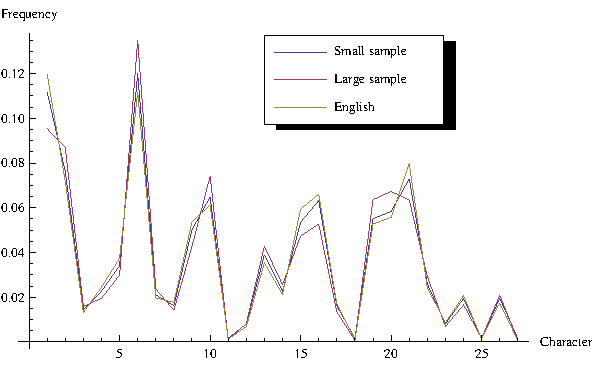
\includegraphics[width=0.9\textwidth]{figures/frequencies-bychar.pdf}
\caption[Plot of character frequencies by frequency]{The character frequencies of the small and large encoded samples, as well as the English target distribution sorted by character.}
\label{FIGURE_frequencies-bytop}
\end{figure}

\begin{figure}
\centering
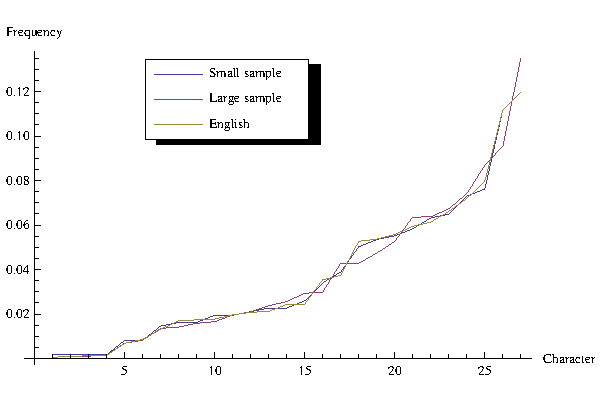
\includegraphics[width=0.9\textwidth]{figures/frequencies-bytop.pdf}
\caption[Plot of character frequencies by character]{The character frequencies of the small and large encoded samples, as well as the English target distribution sorted by frequency.}
\label{FIGURE_frequencies-bychar}
\end{figure}

\subsubsection{Technical Details}
The probabilistic encoder is open-source and freely available, licensed under the Mozilla Public License version 2 which is GPL compatible. The source code is available at \url{https://www.riebart.ca/hg/probcode} for download and use under the MPL2 license terms. The source code compiles on Unix and other POSIX based systems sych as Cygwin on Windows.

The encoding and decoding processes can be broken up into two steps; probability distribution analysis and then the actual conversion. The analysis of the distribution is the same for both the encoding and decoding operations, however the encoding operation is somewhat more involved than the decoding operation from an algorithmic point of view.

The probability distribution is analyzed in order to map each element of the distribution (character, word, etc$\ldots$) to a string of bits. An assumption is made that all bit strings of a given length are equally likely to appear in the high-entropy source, and this places a constraint in the output PDF; the most frequent symbol cannot be more frequent than the most frequent symbol in the high-entropy source. That is, no symbol in the output distribution can have a frequency above 50\%. This is considered a fair assumption since in English, the most common letter has a frequency of approximately 11\%.

The mapping from symbol to bit string is done by sorting the distribution from most to least frequent, and then selecting a shortest available bit string of a length that has an expected occurrence rate not less than the symbol's occurrence rate in the output distribution. For example, the bit string to symbol mapping for the English unigram encoding sample is given in Table \ref{TABLE_unigrammapping} along with the approximate frequency of the letters in English text.

Observe that it is possible to make a tradeoff between encoding accuracy (that is, how accurately the output matches the desired distribution) and encoding efficiency (that is, the ratio between output and input size with higher ratios indicating a less efficient encoding) by tuning the bit string mapping. More accurate mappings result from choosing shorter bit strings (Table \ref{TABLE_unigrammapping} chooses the shortest possible bit string mappings and achieves an efficency factor of approximately 3.3) with more efficient mappings sacrificing accuracy for efficiency. Figure \ref{FIGURE_encoding-accvseff} shows the frequencies of the English target distribution along with the most efficient encoding and the most accurate encoding. The efficient coding in that figure achieves a factor of 

Once the mapping has been built, and the various lookup tables built, the encoding or decoding process can begin. For encoding, a table is maintained that keeps track of how many times each symbol in the desired distribution has been output. The purpose of this table is to facilitate the greedy selection of symbols in order to ensure that one symbol is not chosen more often than is necessary and that those symbols that are farthest from meeting their quota in the output stream get preferential selection when the input bits match their mapping.

\begin{table}
\centering
\begin{tabular}{ c | c | c }
Character&Bit-String&Count\\
\hline
$<$\emph{space}$>$&1          &0.11965   \\
e&0    &0.111823  \\
t&11    &0.0797253\\
a&01    &0.0718989\\
o&10    &0.0660886\\
i&00    &0.0613258\\
n&111    &0.0594154\\
s&011    &0.0557003\\
h&101    &0.0536491\\
r&001    &0.0527071\\
d&110    &0.0374417\\
l&010    &0.0354345\\
c&100    &0.0244916\\
u&000    &0.0242803\\
m&0011    &0.0211814\\
w&1101    &0.0207765\\
f&0101    &0.0196144\\
g&1001    &0.0177392\\
y&0001    &0.0173783\\
p&1110    &0.0169821\\
b&0110    &0.013135\\
v&1010    &0.00860991\\
k&0010    &0.00679637\\
j&1100    &0.00134695\\
x&0100    &0.00132054\\
q&1000    &0.000836341\\
z&0000    &0.000651466\\
\end{tabular}
\caption[English character bit-string mapping]{Bit-string mapping for English characters and their frequency for comparison.}
\label{TABLE_unigrammapping}
\end{table}


\section{Euclidean Distance Between Queries}
\label{querydistance}

\newpage
%\nocite{*} 
%\printbibliography
\bibliography{../Reference/bibliography}{}

% \chapter{Problem Statement}
% 
% As networks increase in capacity and more applications are producing traffic
% across the same network connection, the heterogeneity of the traffic on these
% links is increasing. With this increasing diversity in network traffic comes
% an
% ever widening range of acceptable behaviour patterns which results in a very
% hostile and complicated environment for anomaly detection algorithms.
% 
% The goal of this research is to investigate the feasibility of detecting DNS
% tunnels in near real time at high throughput on a complex network link. This
% detection method should also be robust against known methods of avoiding
% existing techniques.

% As computing technology has evolved, the amount of information that needs to be
% protected has grown with it. In 2012, a small ISP (Internet Service Provider)
% that serves less than ten thousand clients can move several terabytes of data
% per day\footnote{YouTube video at a resolution of 720p is encoded at a bitrate
% of approximately 2.5Mbps which translates into approximately fifty megabytes for
% a three minute video. If a average person watches four such videos in a day,
% then ten thousand clients can produce two terabytes of traffic in a day.}.
% 
% Included in this is data generated by hundreds, if not thousands, of unique
% applications including web browsers, operating systems, video games,
% communication programs, office programs and machine-to-machine communications.
% It is important to realize that each web application (GMail, Yahoo mail, Google
% Docs, YouTube, etc...) behaves in this respect as a unique application. Each
% type of traffic from each application has its own specific pattern that
% describes the traffic it produces under normal circumstances and deviations from
% this pattern contain important information.
% 
% The problem of identifying what portions of the data are either malicious or
% otherwise abnormal becomes one of both scale and discrimination. When looking at
% network links sufficiently busy to supply enough information for analysis, there
% is also a great deal of unrelated traffic that needs to be filtered out in order
% to ensure an accurate result. Being discriminatory enough detect relatively rare
% events\footnote{A DNS tunnel, for example, can be as few as ten to twenty
% packets within billions over a day.} without incurring a large number of false
% positive is essential for an effective detection method.
% 
% Covert communication channels can fall into the category of a 'needle in a hay
% stack', or they can be very obvious but this depends on, primarily, how much
% data they are moving. The more data that is being moved across a covert channel,
% the more likely it is to show up as an anomaly due to the number of packets and
% the proportion of the total traffic it represents.
% 
% Covert channels can be formed over any existing protocol or messaging system,
% but need not require one. One example of a covert channel that does not use
% existing protocols or data transmission mechanisms is called a \emph{timing
% channel}. Timing channels utilize some element of timing to encode and transmit
% information. For example, a timing channel can be formed by encoding information
% sent to remote computers by modifying the delay between packets.

% In order to be able to detect these anomalies at a large scale, and to reduce
% the number of devices performing the analysis on the network, the point at which
% the interception is done needs to be moved closer to the centre of the network.
% Throughput on a given link increase rapidly as the chosen link gets closer to
% the centre of the network, due to aggregation of traffic. 
% 
% Sifting through gigabits of traffic becomes a very computationally expensive
% problem; one which is normally solved by applying more, or specialized,
% hardware\footnote{See proprietary solutions, such as those offered by
% TippingPoint, which employ specialized hardware components such as ASICs and
% FPGAs to improve performance. Other vendors, such as Wedge Networks products,
% improve performance by exploiting the ability to perform portions of its
% workload in parallel and add more commodity processors.}. In order to combat
% this inevitable march of requirements, 

\end{document}